\documentclass[11pt,a4paper]{article}
\usepackage[utf8]{inputenc}
\usepackage{amsmath,amssymb}
\usepackage{color}
\usepackage{graphicx}
\usepackage{hyperref}
\usepackage{url}

% Configuracion de margenes estandar A4
\setlength{\textwidth}{16.5cm}
\setlength{\textheight}{24.0cm}
\setlength{\oddsidemargin}{0.0cm}
\setlength{\evensidemargin}{0.0cm}
\setlength{\topmargin}{-1.2cm}
\setlength{\parindent}{0pt}
\setlength{\parskip}{6pt}

% Definicion de colores para enlaces y destacados
\definecolor{navyblue}{rgb}{0.05, 0.15, 0.45}
\definecolor{darkgreen}{rgb}{0.08, 0.40, 0.12}
\definecolor{darkred}{rgb}{0.55, 0.10, 0.10}
\definecolor{boxbg}{rgb}{0.96, 0.97, 0.99}

\hypersetup{
    colorlinks=true,
    linkcolor=navyblue,
    citecolor=darkgreen,
    urlcolor=navyblue,
    pdftitle={Plan y Guia Tecnica: Reconstruccion 3D por Redes Neuronales en gpr3d},
    pdfauthor={Proyecto SignalHandler / gpr3d - IA Team}
}

\renewcommand{\labelitemi}{$\bullet$}
\renewcommand{\labelitemii}{$-$}
\renewcommand{\labelitemiii}{$\ast$}
\renewcommand{\labelitemiv}{$\cdot$}

\begin{document}

% -----------------------------------------------------------------------------
% PORTADA
% -----------------------------------------------------------------------------
\begin{center}
    {\LARGE \textbf{Plan y Gu{\'\i}a T{\'e}cnica de Implementaci{\'o}n:\\[0.2cm] Reconstrucci{\'o}n 3D de Formas Reales mediante Redes Neuronales y Neural SDF en \texttt{gpr3d}}}\\[0.4cm]
    {\Large \textbf{De la Aproximaci{\'o}n Determinista a la Morfolog{\'\i}a de Alta Fidelidad por Deep Learning y Physics-Informed Neural Networks}}\\[0.3cm]
    \rule{\textwidth}{1.2pt}\\[0.2cm]
    \textbf{Proyecto:} \texttt{SignalHandler} (\textit{gpr3d::ai}) \quad $\bullet$ \quad \textbf{Fecha:} Noviembre 2026 \quad $\bullet$ \quad \textbf{Est{\'a}ndar:} C++20 / ONNX Runtime / PyTorch\\
    \rule{\textwidth}{0.6pt}
\end{center}

\vspace{0.2cm}
\tableofcontents
\vspace{0.4cm}
\hrule
\vspace{0.4cm}

% -----------------------------------------------------------------------------
% SECCION 1: VISION GENERAL Y PARADIGMA HIBRIDO
% -----------------------------------------------------------------------------
\section{Visi{\'o}n General: El Salto de Formas Param{\'e}tricas a Geometr{\'\i}as Reales}

El motor actual de \texttt{gpr3d} genera objetos tridimensionales utilizando primitivas anal{\'\i}ticas geom{\'e}tricas: cilindros param{\'e}tricos de radio uniforme $r$ extruidos a lo largo de ejes de tuber{\'\i}a (triedro de Frenet-Serret) y elipsoides regulares para anomal{\'\i}as puntuales.

Aunque este enfoque es matem{\'a}ticamente elegante y robusto para conductos nuevos y perfectos, en la \textbf{infraestructura subterr{\'a}nea real} los objetos presentan morfolog{\'\i}as heterog{\'e}neas y complejas:
\begin{enumerate}
    \item \textbf{Deformaciones mec{\'a}nicas y aplastamientos:} Tuber{\'\i}as pl{\'a}sticas de PVC/HDPE o conductos de alcantarillado que han colapsado el{\'\i}pticamente bajo el peso del tr{\'a}fico vehicular.
    \item \textbf{Accesorios e interferencias angulares:} Codos a $45^\circ$ y $90^\circ$, derivaciones en T, reducciones de di{\'a}metro, v{\'a}lvulas y cajas de empalme prism{\'a}ticas de telecomunicaciones.
    \item \textbf{Cuerpos y cavidades irregulares:} Socavones producidos por fugas de agua, oquedades con superficies rugosas y bloques de roca err{\'a}ticos que envuelven las canalizaciones.
    \item \textbf{L{\'\i}mite de resoluci{\'o}n cl{\'a}sico de Rayleigh:} Dos conductos de fibra {\'o}ptica colocados a menos de $5\text{ cm}$ de distancia se solapan difractivamente en el radargrama, apareciendo como una {\'u}nica masa informe en la f{\'\i}sica cl{\'a}sica.
\end{enumerate}

Para resolver estos desaf{\'\i}os sin sacrificar la rigurosidad f{\'\i}sica, se dise{\~n}a el \textbf{Paradigma H{\'\i}brido F{\'\i}sica Determinista + Deep Learning (PINN + Neural SDF)}, ilustrado en la Figura~\ref{fig:ai_arquitectura}.

\begin{figure}[htbp]
    \centering
    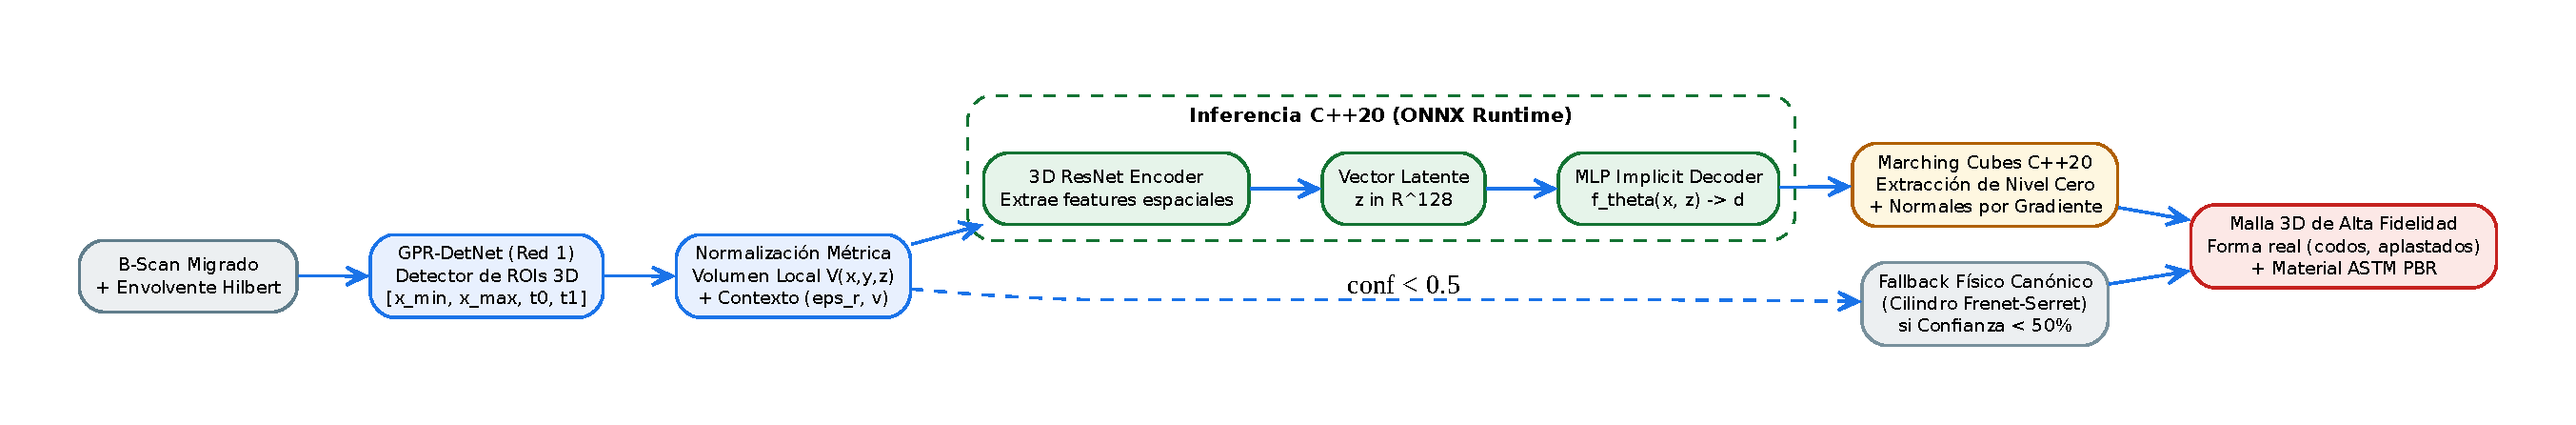
\includegraphics[width=0.95\textwidth]{diagrams/ai_arquitectura_reconstruccion.pdf}
    \caption{Arquitectura del subsistema de Inteligencia Artificial de \texttt{gpr3d} y su acoplamiento con la f{\'\i}sica determinista.}
    \label{fig:ai_arquitectura}
\end{figure}

\subsection{El Principio de Cooperaci{\'o}n H{\'\i}brida}
La red neuronal \textbf{no} debe aprender la f{\'\i}sica desde cero (lo cual requerir{\'\i}a millones de par{\'a}metros y resultar{\'\i}a inestable). El motor en C++20 le proporciona a la IA:
\begin{itemize}
    \item La velocidad real de propagaci{\'o}n $v$ y permitividad $\varepsilon_r$ obtenidas por an{\'a}lisis de semblanza (Sprint 9).
    \item La posici{\'o}n inicial aproximada de los reflectores colapsados mediante migraci{\'o}n de Kirchhoff (Sprint 8).
    \item La polaridad de fase y la clasificaci{\'o}n litol{\'o}gica de material ASTM (Sprint 9).
\end{itemize}
Con esta informaci{\'o}n contextual, la red neuronal se especializa exclusivamente en resolver la \textbf{morfolog{\'\i}a volum{\'e}trica fina a escala sub-longitud de onda}, prediciendo un campo de distancia signada continuo $f_\theta(\mathbf{x}) = d$.

\newpage

% -----------------------------------------------------------------------------
% SECCION 2: FUNDAMENTOS MATEMATICOS Y MAPEO BIBLIOGRAFICO
% -----------------------------------------------------------------------------
\section{Fundamentos Matem{\'a}ticos de Neural SDF y Mapeo Acad{\'e}mico}

\subsection{1. Mapeo a Literatura Est{\'a}ndar Universitaria}
\begin{itemize}
    \item \textbf{\textit{Mathematik} (Tilo Arens et al.)}:
    \begin{itemize}
        \item \textbf{Kapitel 24 \& 25 (\textit{Fl{\"a}chen im Raum und Vektoranalysis})}: Superficies impl{\'\i}citas $F(x, y, z) = 0$, gradiente $\nabla F = (\frac{\partial F}{\partial x}, \frac{\partial F}{\partial y}, \frac{\partial F}{\partial z})$, y vector normal unitario $\mathbf{n} = \nabla F / \|\nabla F\|$.
        \item \textbf{Kapitel 27 (\textit{Partielle Differentialgleichungen})}: Ecuaci{\'o}n Eikonal no lineal $\|\nabla \Phi(\mathbf{x})\| = 1$, propagaci{\'o}n de frentes de onda y geometr{\'\i}a de distancias euclidianas m{\'\i}nimas a conjuntos cerrados.
        \item \textbf{Kapitel 28 (\textit{Numerische Optimierung})}: M{\'e}todo de descenso de gradiente estoc{\'a}stico (SGD), aproximaci{\'o}n por m{\'\i}nimos cuadrados no lineales y regularizaci{\'o}n de Tikhonov.
    \end{itemize}
    \item \textbf{\textit{Physik f{\"u}r Wissenschaftler und Ingenieure} (Tipler \& Mosca)}:
    \begin{itemize}
        \item \textbf{Kapitel 15 (\textit{Wellen und Beugung})}: Dispersi{\'o}n de ondas electromagn{\'e}ticas en obst{\'a}culos de dimensiones comparables a la longitud de onda ($\lambda = v / f$).
        \item \textbf{Kapitel 31 (\textit{Optik})}: Criterio de Rayleigh para resoluci{\'o}n l{\'\i}mite angular y espacial ($\Delta x_{\min} \approx 0.61 \lambda / \text{NA}$).
    \end{itemize}
    \item \textbf{Literatura Fundamental de Deep Learning y Redes Guiadas por la F{\'\i}sica (PINN)}:
    \begin{itemize}
        \item \textbf{Goodfellow, Bengio \& Courville (\textit{Deep Learning}, MIT Press)}: Convoluciones 3D, funciones de activaci{\'o}n no lineales (ReLU, Sine/SIREN, GELU) y optimizador AdamW con regularizaci{\'o}n de pesos.
        \item \textbf{Raissi, Perdikaris \& Karniadakis (2019, \textit{Physics-Informed Neural Networks}, J. Comp. Phys.)}: Penalizaci{\'o}n de residuos de ecuaciones diferenciales parciales (EDP) en la funci{\'o}n de p{\'e}rdida mediante diferenciaci{\'o}n autom{\'a}tica.
        \item \textbf{Gropp, Yariv, Haim, Atzmon \& Lipman (2020, \textit{Implicit Geometric Regularization for Learning Shapes}, NeurIPS)}: Regularizaci{\'o}n geom{\'e}trica impl{\'\i}cita mediante la condici{\'o}n eikonal $\|\nabla_\mathbf{x} f_\theta(\mathbf{x})\| = 1$.
        \item \textbf{Park, Florence, Straub, Newcombe \& Lovegrove (2019, \textit{DeepSDF: Learning Continuous Signed Distance Functions}, CVPR)}: Representaci{\'o}n continua de formas 3D condicionadas por c{\'o}digos latentes.
    \end{itemize}
    \item \textbf{\textit{C++ professionell anwenden} (Ulrich Breymann)}:
    \begin{itemize}
        \item \textbf{Kapitel 7, 8 \& 11}: Gesti{\'o}n de memoria contigua en C++20 con \texttt{std::span}, construcci{\'o}n de tensores planos sin copias intermedias y estructuras de datos para mallas triangulares.
        \item \textbf{Kapitel 18 (\textit{C-Bibliotheken})}: Integraci{\'o}n del runtime de inferencia nativo \texttt{onnxruntime-cxx} con punteros inteligentes RAII y ejecuci{\'o}n sin int{\'e}rprete de Python.
    \end{itemize}
\end{itemize}

\subsection{2. La Representaci{\'o}n Geom{\'e}trica por Neural SDF}
En lugar de discretizar el espacio en cuadr{\'\i}culas de p{\'\i}xeles o p{\'o}xeles volum{\'e}tricos (v{\'o}xeles), una \textbf{Funci{\'o}n de Distancia Signada Neuronal (Neural SDF)} modela el objeto como un campo continuo parametrizado por una red neuronal profunda $f_\theta$:
\begin{equation}
    f_\theta : \mathbb{R}^3 \times \mathbb{R}^k \to \mathbb{R}, \qquad f_\theta(\mathbf{x}, \mathbf{z}) = d
\end{equation}
donde $\mathbf{x} = (x, y, z)$ es un punto de consulta en el espacio tridimensional en metros, $\mathbf{z} \in \mathbb{R}^{128}$ es el vector latente que describe las caracter{\'\i}sticas del objeto detectado en el radargrama, y $d$ es la distancia euclidiana signada con la convenci{\'o}n (ver Figura~\ref{fig:neural_sdf}):
\begin{equation}
    d = \begin{cases}
        < 0 & \text{si } \mathbf{x} \text{ se encuentra en el interior del objeto (ej. n{\'u}cleo del tubo)} \\
        = 0 & \text{si } \mathbf{x} \text{ se encuentra sobre la superficie o pared f{\'\i}sica real} \\
        > 0 & \text{si } \mathbf{x} \text{ se encuentra en el exterior (ej. suelo o estrato circundante)}
    \end{cases}
\end{equation}

\begin{figure}[htbp]
    \centering
    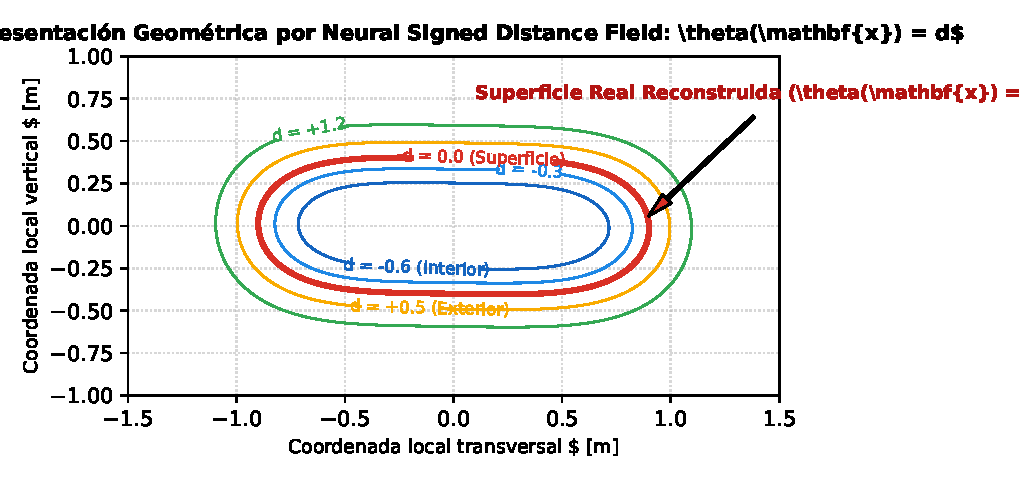
\includegraphics[width=0.78\textwidth]{diagrams/neural_sdf_concepto.pdf}
    \caption{Curvas de nivel del campo escalar continuo predicho por Neural SDF. La superficie f{\'\i}sica real se extrae evaluando el conjunto de nivel cero $f_\theta(\mathbf{x}) = 0$.}
    \label{fig:neural_sdf}
\end{figure}

\subsection{3. Propiedades Matem{\'a}ticas Clave del Neural SDF}
\begin{enumerate}
    \item \textbf{Resoluci{\'o}n Infinita:} Al ser una funci{\'o}n continua $f_\theta$, no existe un tama{\~n}o m{\'\i}nimo de p{\'\i}xel. Se puede evaluar la malla poligonal con cualquier nivel de detalle arbitrario (paso de $5\text{ mm}$ o $1\text{ mm}$).
    \item \textbf{Topolog{\'\i}a Arbitraria sin Costuras:} A diferencia de los tubos param{\'e}tricos que solo pueden modelar cilindros simples no bifurcados, un conjunto de nivel cero $f_\theta(\mathbf{x}) = 0$ puede representar de forma nativa codos, uniones en T, cajas de registro huecas o zanjas irregulares sin costuras matem{\'a}ticas ni desgarros de malla.
    \item \textbf{C{\'a}lculo Anal{\'\i}tico Exacto de Normales por Gradiente:}
    La normal unitaria exterior a la superficie en cualquier punto de la pared se obtiene directamente evaluando el gradiente del campo SDF:
    \begin{equation}
        \mathbf{n}(\mathbf{x}) = \frac{\nabla_\mathbf{x} f_\theta(\mathbf{x})}{\|\nabla_\mathbf{x} f_\theta(\mathbf{x})\|}
    \end{equation}
    lo que produce un sombreado suave (\textit{smooth shading}) perfecto para renderizado PBR en motores 3D sin tener que promediar tri{\'a}ngulos vecinos ruidosos.
\end{enumerate}

\begin{figure}[htbp]
    \centering
    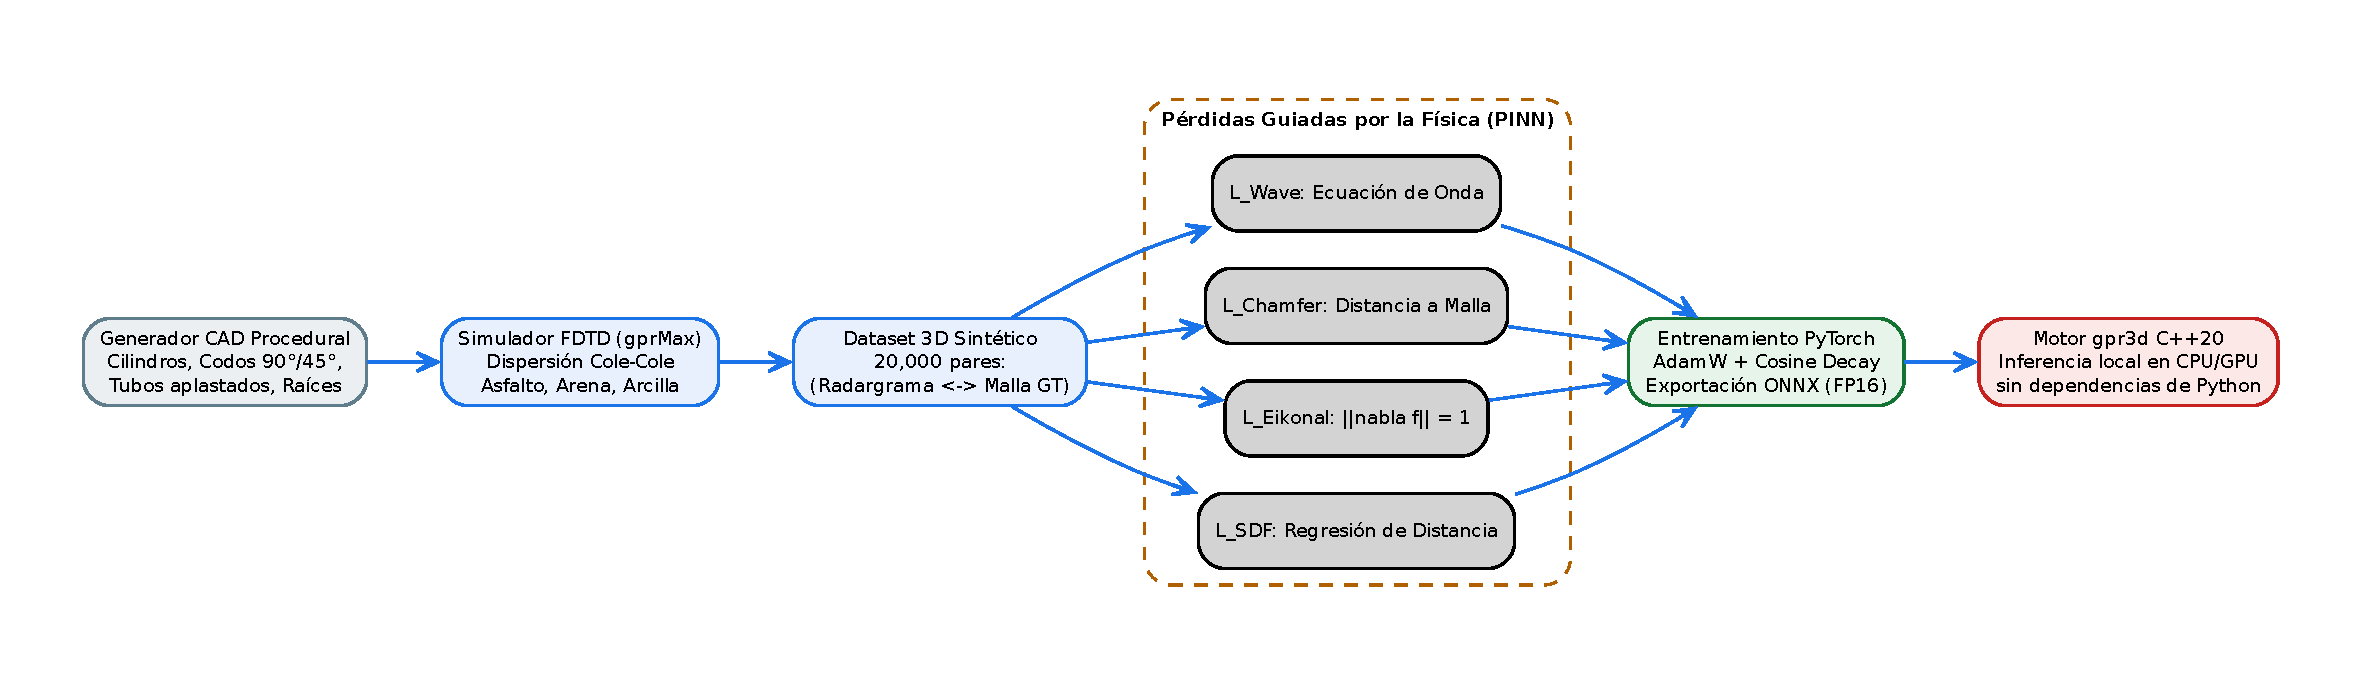
\includegraphics[width=0.92\textwidth]{diagrams/pipeline_entrenamiento_ia.pdf}
    \caption{Flujo de simulaci{\'o}n electromagn{\'e}tica FDTD, entrenamiento con p{\'e}rdidas f{\'\i}sicas PINN y exportaci{\'o}n a ONNX C++20.}
    \label{fig:pipeline_entrenamiento}
\end{figure}


% =============================================================================
% SPRINT IA-0: INFRAESTRUCTURA DE INFERENCIA NATIVA C++20 CON ONNX RUNTIME
% =============================================================================
\section{Sprint IA-0: Infraestructura de Inferencia Nativa C++20 con ONNX Runtime}

\subsection{1. Qu{\'e} Estudiar en la Literatura T{\'e}cnica}
\begin{itemize}
    \item \textbf{\textit{C++ professionell anwenden} (Ulrich Breymann)}:
    \begin{itemize}
        \item \textbf{Kapitel 7 \& 8 (\textit{Speicherverwaltung und Smart Pointer})}: Gesti{\'o}n RAII de entornos de ejecuci{\'o}n nativos, encapsulaci{\'o}n de \texttt{Ort::Env}, \texttt{Ort::Session} y liberaci{\'o}n determinista de memoria.
        \item \textbf{Kapitel 11 (\textit{Containers und Views en C++20})}: Uso estricto de \texttt{std::span<const float>} para referenciar tensores planos sin realizar copias innecesarias de b{\'u}feres de radargramas.
        \item \textbf{Kapitel 18 (\textit{Integration externer C/C++ Bibliotheken})}: Vinculaci{\'o}n din{\'a}mica y est{\'a}tica con la API en C de \texttt{onnxruntime}.
    \end{itemize}
    \item \textbf{Documentaci{\'o}n Oficial de ONNX Runtime C++ API}:
    \begin{itemize}
        \item Creaci{\'o}n de \texttt{Ort::MemoryInfo} para b{\'u}feres de CPU/GPU, configuraci{\'o}n de hilos intra e inter-op (\texttt{SetIntraOpNumThreads}), y asignadores de memoria (\texttt{Ort::AllocatorWithDefaultOptions}).
    \end{itemize}
\end{itemize}

\subsection{2. Por Qu{\'e} Hay que Implementarlo}
En el {\'a}mbito industrial y de ingenier{\'\i}a civil sobre el terreno (tablets de campo, estaciones de trabajo embarcadas en furgonetas geof{\'\i}sicas), \textbf{es inaceptable depender de int{\'e}rpretes de Python o servidores de microservicios externos}:
\begin{enumerate}
    \item \textbf{Latencia y Determinismo:} Python introduce el Global Interpreter Lock (GIL) y sobrecargas de recolecci{\'o}n de basura (GC) que impiden garantizar tiempos de respuesta deterministas en el procesado en l{\'\i}nea.
    \item \textbf{Huella de Memoria:} Un entorno de Python con PyTorch cargado consume m{\'a}s de $1.2\text{ GB}$ de RAM simplemente al importar m{\'o}dulos. El runtime nativo de ONNX en C++20 consume menos de $35\text{ MB}$ de RAM b{\'a}sica.
    \item \textbf{Despliegue Cero Dependencias:} La aplicaci{\'o}n \texttt{gpr3d} debe compilarse como un {\'u}nico binario aut{\'o}nomo (\textit{standalone}) que pueda ejecutarse en cualquier sistema Linux/Windows sin requerir instalaciones de Conda, pip o paquetes de terceros.
\end{enumerate}

\subsection{3. Tareas Paso a Paso de Implementaci{\'o}n}

\begin{enumerate}
    \item \textbf{Definici{\'o}n de la cabecera del motor de inferencia nativo}:
    Crear el archivo \texttt{include/gpr3d/ai/inference\_engine.hpp}:
\begin{verbatim}
#pragma once
#include <string>
#include <vector>
#include <memory>
#include <span>
#include <onnxruntime_cxx_api.h>

namespace gpr3d::ai {

struct TensorShape {
    std::vector<int64_t> dims;
    size_t total_elements() const {
        size_t count = 1;
        for (auto d : dims) count *= static_cast<size_t>(d);
        return count;
    }
};

class OnnxInferenceEngine {
public:
    explicit OnnxInferenceEngine(const std::string& model_path, int num_threads = 4);
    ~OnnxInferenceEngine() = default;

    // Ejecucion de inferencia con memoria continua sin copias
    std::vector<float> run(
        std::span<const float> input_tensor,
        const TensorShape& input_shape,
        const std::string& input_name,
        const std::string& output_name
    );

    // Consulta de metadatos del modelo exportado
    [[nodiscard]] TensorShape get_input_shape(size_t index = 0) const;
    [[nodiscard]] TensorShape get_output_shape(size_t index = 0) const;

private:
    Ort::Env env_;
    Ort::SessionOptions session_options_;
    std::unique_ptr<Ort::Session> session_;
    Ort::MemoryInfo memory_info_;
    std::vector<std::string> input_names_;
    std::vector<std::string> output_names_;
};

} // namespace gpr3d::ai
\end{verbatim}

    \item \textbf{Implementaci{\'o}n de la l{\'o}gica de sesi{\'o}n y pasarela de memoria}:
    Crear el archivo \texttt{src/ai/inference\_engine.cpp}:
\begin{verbatim}
#include "gpr3d/ai/inference_engine.hpp"
#include <stdexcept>
#include <numeric>

namespace gpr3d::ai {

OnnxInferenceEngine::OnnxInferenceEngine(const std::string& model_path, int num_threads)
    : env_(ORT_LOGGING_LEVEL_WARNING, "gpr3d_ai"),
      memory_info_(Ort::MemoryInfo::CreateCpu(OrtArenaAllocator, OrtMemTypeDefault)) {
    session_options_.SetIntraOpNumThreads(num_threads);
    session_options_.SetGraphOptimizationLevel(GraphOptimizationLevel::ORT_ENABLE_ALL);
    session_ = std::make_unique<Ort::Session>(env_, model_path.c_str(), session_options_);
    
    // Extraccion de nombres de nodos de entrada y salida
    Ort::AllocatorWithDefaultOptions allocator;
    size_t num_inputs = session_->GetInputCount();
    for (size_t i = 0; i < num_inputs; ++i) {
        auto name_ptr = session_->GetInputNameAllocated(i, allocator);
        input_names_.emplace_back(name_ptr.get());
    }
    size_t num_outputs = session_->GetOutputCount();
    for (size_t i = 0; i < num_outputs; ++i) {
        auto name_ptr = session_->GetOutputNameAllocated(i, allocator);
        output_names_.emplace_back(name_ptr.get());
    }
}

std::vector<float> OnnxInferenceEngine::run(
    std::span<const float> input_tensor,
    const TensorShape& input_shape,
    const std::string& input_name,
    const std::string& output_name
) {
    if (input_tensor.size() != input_shape.total_elements()) {
        throw std::invalid_argument("El tamano del span no coincide con la forma del tensor.");
    }
    
    // Creacion del tensor envolviendo directamente el puntero de datos (zero-copy)
    Ort::Value input_val = Ort::Value::CreateTensor<float>(
        memory_info_,
        const_cast<float*>(input_tensor.data()),
        input_tensor.size(),
        input_shape.dims.data(),
        input_shape.dims.size()
    );

    const char* in_names[] = { input_name.c_str() };
    const char* out_names[] = { output_name.c_str() };

    auto output_tensors = session_->Run(
        Ort::RunOptions{nullptr},
        in_names,
        &input_val,
        1,
        out_names,
        1
    );

    float* out_data = output_tensors.front().GetTensorMutableData<float>();
    auto info = output_tensors.front().GetTensorTypeAndShapeInfo();
    size_t total_out = info.GetElementCount();

    return std::vector<float>(out_data, out_data + total_out);
}

TensorShape OnnxInferenceEngine::get_input_shape(size_t index) const {
    auto type_info = session_->GetInputTypeInfo(index);
    auto shape_info = type_info.GetTensorTypeAndShapeInfo();
    return TensorShape{ shape_info.GetShape() };
}

TensorShape OnnxInferenceEngine::get_output_shape(size_t index) const {
    auto type_info = session_->GetOutputTypeInfo(index);
    auto shape_info = type_info.GetTensorTypeAndShapeInfo();
    return TensorShape{ shape_info.GetShape() };
}

} // namespace gpr3d::ai
\end{verbatim}

    \item \textbf{Configuraci{\'o}n en CMake}:
    A{\~n}adir a \texttt{CMakeLists.txt} la b{\'u}squeda o descarga autom{\'a}tica de \texttt{onnxruntime} y el enlace del objetivo \texttt{gpr3d\_ai}.
\end{enumerate}

\subsection{4. Prueba de Verificaci{\'o}n Num{\'e}rica}
Implementar \texttt{test/test\_ai\_inference\_engine.cpp}:
\begin{enumerate}
    \item Crear un modelo sint{\'e}tico ONNX que ejecute una operaci{\'o}n elemental $y = 2.0x + 1.0$ para un tensor de dimensi{\'o}n $(1, 3)$.
    \item Instanciar \texttt{OnnxInferenceEngine} con dicho modelo.
    \item Pasar como entrada el vector $\{1.0, 2.0, 3.0\}$.
    \item \textbf{Criterio de Aprobaci{\'o}n}: La salida debe coincidir exactamente con $\{3.0, 5.0, 7.0\}$ con un error absoluto m{\'a}ximo inferior a $10^{-6}$, y el tiempo de ejecuci{\'o}n debe ser menor a $0.5\text{ ms}$.
\end{enumerate}

\newpage

% =============================================================================
% SPRINT IA-1: GENERADOR SINTETICO DE GEMELOS DIGITALES FDTD CON GPRMAX
% =============================================================================
\section{Sprint IA-1: Generador Sint{\'e}tico de Gemelos Digitales FDTD con gprMax}

\subsection{1. Qu{\'e} Estudiar en la Literatura T{\'e}cnica}
\begin{itemize}
    \item \textbf{\textit{Physik f{\"u}r Wissenschaftler und Ingenieure} (Tipler \& Mosca)}:
    \begin{itemize}
        \item \textbf{Kapitel 20 (\textit{Elektromagnetische Schwingungen und Wellen})}: Ecuaciones de Maxwell en el dominio del tiempo:
        \begin{equation}
            \nabla \times \mathbf{E} = -\mu \frac{\partial \mathbf{H}}{\partial t}, \qquad \nabla \times \mathbf{H} = \sigma \mathbf{E} + \varepsilon \frac{\partial \mathbf{E}}{\partial t}
        \end{equation}
        \item \textbf{Discretizaci{\'o}n de Yee}: Desfase espacial y temporal de componentes el{\'e}ctricas y magn{\'e}ticas en celdas c{\'u}bicas $\Delta x = \Delta y = \Delta z$.
    \end{itemize}
    \item \textbf{\textit{Mathematik} (Tilo Arens et al.)}:
    \begin{itemize}
        \item \textbf{Kapitel 27 (\textit{Partielle Differentialgleichungen})}: Condici{\'o}n de estabilidad de Courant-Friedrichs-Lewy (CFL) en 3D:
        \begin{equation}
            \Delta t \le \frac{1}{c \sqrt{\frac{1}{\Delta x^2} + \frac{1}{\Delta y^2} + \frac{1}{\Delta z^2}}}
        \end{equation}
    \end{itemize}
    \item \textbf{Documentaci{\'o}n de gprMax (Warren et al.)}:
    \begin{itemize}
        \item Definici{\'o}n de capas Perfectly Matched Layers (PML) de absorci{\'o}n, antenas de pulso Ricker dipolar hertziano y fractales de rugosidad ed{\'a}fica de Peplinski.
    \end{itemize}
\end{itemize}

\subsection{2. Por Qu{\'e} Hay que Implementarlo}
El principal obst{\'a}culo para aplicar Deep Learning a datos de radar de subsuelo en la industria civil es la \textbf{carencia de datos reales anotados con certeza milim{\'e}trica}:
\begin{enumerate}
    \item \textbf{Imposibilidad de Excavaci{\'o}n Destructiva Continua:} No es viable excavar zanjas destructivas en v{\'\i}as p{\'u}blicas para medir con l{\'a}ser 3D la forma exacta de cada tuber{\'\i}a enterrada simplemente para etiquetar un dataset.
    \item \textbf{Representatividad Estad{\'\i}stica de Defectos Cr{\'\i}ticos:} Los casos m{\'a}s peligrosos (tuber{\'\i}as de gas aplastadas por compactaci{\'o}n, socavones oquedades bajo pavimento, codos que cruzan en {\'a}ngulo oblicuo) ocurren de manera espor{\'a}dica. Un modelo entrenado solo con datos de campo t{\'\i}picos jam{\'a}s aprender{\'a} a reconocer fallas geom{\'e}tricas raras.
    \item \textbf{Gemelo Digital FDTD Riguroso:} Generar 15,000 pares de entrenamiento mediante FDTD (\texttt{gprMax}) donde conocemos la malla 3D exacta del CAD procedural permite entrenar redes con una precisi{\'o}n absoluta, resolviendo la f{\'\i}sica electromagn{\'e}tica completa (reflexiones m{\'u}ltiples, difracci{\'o}n y atenuaci{\'o}n de suelos).
\end{enumerate}

\subsection{3. Tareas Paso a Paso de Implementaci{\'o}n}

\begin{enumerate}
    \item \textbf{Desarrollo del generador procedural de geometr{\'\i}as CAD}:
    Crear el script en Python \texttt{scripts/ai/procedural\_cad\_generator.py}:
\begin{verbatim}
import numpy as np
import trimesh

def create_deformed_pipe(length=2.0, radius=0.10, crush_ratio=0.6, bend_angle=0.0):
    # Genera un tubo con seccion deformada elipticamente y posible curvatura axial.
    # crush_ratio: razon entre el radio vertical comprimido y el radio horizontal.
    n_theta, n_z = 32, 64
    theta = np.linspace(0, 2*np.pi, n_theta)
    z = np.linspace(-length/2, length/2, n_z)
    
    rx = radius / np.sqrt(crush_ratio)
    ry = radius * np.sqrt(crush_ratio)
    
    vertices = []
    for zi in z:
        # Deformacion axial (codo o comba)
        offset_y = (zi**2 / (length/2)**2) * np.tan(np.radians(bend_angle)) * 0.2
        for th in theta:
            x = rx * np.cos(th)
            y = ry * np.sin(th) + offset_y
            vertices.append([x, y, zi])
            
    # Ensamblado de caras poligonales
    faces = []
    for i in range(n_z - 1):
        for j in range(n_theta):
            p1 = i * n_theta + j
            p2 = i * n_theta + (j + 1) % n_theta
            p3 = (i + 1) * n_theta + (j + 1) % n_theta
            p4 = (i + 1) * n_theta + j
            faces.append([p1, p2, p3])
            faces.append([p1, p3, p4])
            
    mesh = trimesh.Trimesh(vertices=vertices, faces=faces)
    return mesh
\end{verbatim}

    \item \textbf{Automatizaci{\'o}n de simulaciones FDTD batch en gprMax}:
    Crear \texttt{scripts/ai/gprmax\_batch\_runner.py}:
\begin{verbatim}
import os
import subprocess
import h5py
import numpy as np

def generate_gprmax_in(filepath, domain=(1.5, 1.5, 1.0), dx=0.005, f_c=800e6,
                       eps_soil=9.0, sigma_soil=0.005, object_type="pipe", mesh_file=""):
    dt = dx / (3e8 * np.sqrt(3)) * 0.99
    with open(filepath, 'w') as f:
        f.write(f"#domain: {domain[0]} {domain[1]} {domain[2]}\n")
        f.write(f"#dx_dy_dz: {dx} {dx} {dx}\n")
        f.write(f"#time_window: 25e-9\n")
        f.write(f"#material: {eps_soil} {sigma_soil} 1.0 0.0 soil\n")
        f.write(f"#waveform: ricker 1.0 {f_c} my_ricker\n")
        f.write(f"#hertzian_dipole: z 0.1 0.75 0.9 my_ricker\n")
        f.write(f"#rx: 0.24 0.75 0.9\n")
        f.write(f"#geometry_objects_read: 0.1 0.1 0.1 {mesh_file} soil\n")
\end{verbatim}

    \item \textbf{Constructor del dataset unificado HDF5}:
    Crear \texttt{scripts/ai/dataset\_builder.py} para empaquetar vol{\'u}menes B-scan/C-scan sintetizados, nubes de puntos con distancias SDF pre-calculadas y metadatos litol{\'o}gicos en \texttt{data/training\_dataset.h5}.
\end{enumerate}

\subsection{4. Prueba de Verificaci{\'o}n Num{\'e}rica}
\begin{enumerate}
    \item Ejecutar una simulaci{\'o}n de prueba con un tubo cil{\'\i}ndrico de di{\'a}metro conocido $d = 160\text{ mm}$ a $0.80\text{ m}$ de profundidad en suelo con $\varepsilon_r = 9.0$.
    \item Medir el tiempo de arribo de doble v{\'\i}a en la traza central del radargrama simulado:
    \begin{equation}
        v = \frac{c}{\sqrt{9.0}} = 0.10\text{ m/ns}, \qquad t = \frac{2 \times 0.80\text{ m}}{0.10\text{ m/ns}} = 16.0\text{ ns}
    \end{equation}
    \item \textbf{Criterio de Aprobaci{\'o}n}: El pico principal de reflexi{\'o}n en el archivo HDF5 generado debe situarse exactamente en $t = 16.0\text{ ns} \pm 0.15\text{ ns}$, validando la coherencia f{\'\i}sica del simulador.
\end{enumerate}

\newpage

% =============================================================================
% SPRINT IA-2: RED 1 (GPR-DETNET) - DETECTOR 3D DE REGIONES DE INTERES (ROI)
% =============================================================================
\section{Sprint IA-2: Red 1 (GPR-DetNet) - Detector 3D de Regiones de Inter{\'e}s (ROI)}

\subsection{1. Qu{\'e} Estudiar en la Literatura T{\'e}cnica}
\begin{itemize}
    \item \textbf{\textit{Deep Learning} (Goodfellow, Bengio \& Courville)}:
    \begin{itemize}
        \item \textbf{Kapitel 9 (\textit{Faltungsnetzwerke / Convolutional Networks})}: Convoluciones 3D para procesamiento de vol{\'u}menes espacio-temporales ($x, y, t$), capas de agrupamiento tridimensional (\textit{3D Max Pooling}) y normalizaci{\'o}n por lotes (\textit{Batch Normalization}).
        \item \textbf{Focal Loss para Detecci{\'o}n de Objetos Raros}:
        \begin{equation}
            \mathcal{L}_{\text{focal}}(p_t) = -\alpha_t (1 - p_t)^\gamma \log(p_t)
        \end{equation}
        dise{\~n}ada para evitar que el 95\% del volumen de suelo homog{\'e}neo y vac{\'\i}o domine el gradiente sobre las anomal{\'\i}as subterr{\'a}neas.
    \end{itemize}
    \item \textbf{\textit{Mathematik} (Tilo Arens et al.)}:
    \begin{itemize}
        \item \textbf{Kapitel 25 (\textit{Lineare Ausgleichsrechnung})}: C{\'a}lculo de intersecci{\'o}n volum{\'e}trica entre prismas rectangulares 3D (\textit{Intersection over Union} - 3D IoU).
    \end{itemize}
\end{itemize}

\subsection{2. Por Qu{\'e} Hay que Implementarlo}
Una cuadr{\'\i}cula completa de prospecci{\'o}n GPR t{\'\i}pica (ej. $20\text{ m} \times 10\text{ m} \times 2.5\text{ m}$) contiene decenas de millones de muestras:
\begin{enumerate}
    \item \textbf{Inviabilidad Computacional de Reconstrucci{\'o}n Global:} Evaluar un campo neuronal continuo SDF en todo el volumen con resoluci{\'o}n de mil{\'\i}metros requerir{\'\i}a evaluar la red neuronal m{\'a}s de $2 \times 10^8$ veces, tardando horas por escaneo.
    \item \textbf{Estrategia Coarse-to-Fine (Detecci{\'o}n Gruesa $\to$ Reconstrucci{\'o}n Fina):} GPR-DetNet act{\'u}a como la etapa gruesa (\textit{coarse stage}): procesa el volumen migrado r{\'a}pidamente mediante convoluciones 3D ligeras y devuelve {\'u}nicamente las cajas envolventes 3D delimitadoras ($[x_{\min}, y_{\min}, z_{\min}, x_{\max}, y_{\max}, z_{\max}]$) y la clase probable (tuber{\'\i}a, caja, oquedad).
    \item \textbf{Enfoque del Presupuesto de C{\'a}lculo:} El motor C++ solo invoca la red densa Neural SDF (Sprint IA-3) dentro de las cajas 3D delimitadas, reduciendo el volumen de consulta en un 98.5\% y permitiendo inferencia interactiva en menos de $1.5\text{ segundos}$.
\end{enumerate}

\subsection{3. Tareas Paso a Paso de Implementaci{\'o}n}

\begin{enumerate}
    \item \textbf{Definici{\'o}n de la arquitectura en PyTorch y p{\'e}rdidas combinadas}:
    Crear el archivo \texttt{scripts/ai/models/gpr\_detnet.py}:
\begin{verbatim}
import torch
import torch.nn as nn
import torch.nn.functional as F

class ResidualBlock3D(nn.Module):
    def __init__(self, channels):
        super().__init__()
        self.conv1 = nn.Conv3d(channels, channels, kernel_size=3, padding=1)
        self.bn1 = nn.BatchNorm3d(channels)
        self.conv2 = nn.Conv3d(channels, channels, kernel_size=3, padding=1)
        self.bn2 = nn.BatchNorm3d(channels)

    def forward(self, x):
        res = x
        x = F.gelu(self.bn1(self.conv1(x)))
        x = self.bn2(self.conv2(x))
        return F.gelu(x + res)

class GPRDetNet(nn.Module):
    # Detector 3D para volumenes de radargramas migrados (Batch, 1, Depth, Height, Width).
    # Salidas:
    #   - classification: probabilidad de presencia de anomalia (Softmax 4 clases).
    #   - bbox_regression: parametros de la caja 3D (cx, cy, cz, w, h, d, theta_yaw).
    def __init__(self, num_classes=4):
        super().__init__()
        self.encoder = nn.Sequential(
            nn.Conv3d(1, 32, kernel_size=5, stride=2, padding=2),
            nn.BatchNorm3d(32),
            nn.GELU(),
            ResidualBlock3D(32),
            nn.Conv3d(32, 64, kernel_size=3, stride=2, padding=1),
            nn.BatchNorm3d(64),
            nn.GELU(),
            ResidualBlock3D(64),
            nn.Conv3d(64, 128, kernel_size=3, stride=2, padding=1),
            nn.BatchNorm3d(128),
            nn.GELU(),
            ResidualBlock3D(128)
        )
        self.cls_head = nn.Conv3d(128, num_classes, kernel_size=1)
        self.box_head = nn.Conv3d(128, 7, kernel_size=1) # 3 centros, 3 dimensiones, 1 yaw

    def forward(self, x):
        feat = self.encoder(x)
        cls_logits = self.cls_head(feat)
        box_preds = self.box_head(feat)
        return cls_logits, box_preds
\end{verbatim}

    \item \textbf{Exportaci{\'o}n a ONNX con perfilado din{\'a}mico}:
    Crear \texttt{scripts/ai/export\_detnet\_onnx.py} para generar \texttt{models/gpr\_detnet.onnx} con dimensiones de batch y volumen din{\'a}micas.

    \item \textbf{Integraci{\'o}n del cliente C++20 para detecci{\'o}n de ROIs}:
    Crear \texttt{include/gpr3d/ai/detnet\_detector.hpp} y \texttt{src/ai/detnet\_detector.cpp} que tome una instancia de \texttt{Grid3D<float>} migrada, invoque el motor \texttt{OnnxInferenceEngine} y filtre las cajas por Non-Maximum Suppression (NMS) 3D.
\end{enumerate}

\subsection{4. Prueba de Verificaci{\'o}n Num{\'e}rica}
Implementar \texttt{test/test\_detnet\_detector.cpp}:
\begin{enumerate}
    \item Generar un volumen de radar sint{\'e}tico de $64 \times 64 \times 64$ muestras conteniendo un reflector hipers{\'o}lico a prop{\'o}sito en la regi{\'o}n $x \in [0.4, 0.6]\text{ m}$, $y \in [0.8, 1.2]\text{ m}$, $z \in [0.5, 0.7]\text{ m}$.
    \item Ejecutar la inferencia de \texttt{DetNetDetector}.
    \item \textbf{Criterio de Aprobaci{\'o}n}: Debe detectarse exactamente una caja envolvente con clasificaci{\'o}n \texttt{PIPE} con una confianza superior al $85\%$, y el centroide predicho debe coincidir con el centro real con un error m{\'a}ximo de posici{\'o}n inferior a $\pm 3\text{ cm}$.
\end{enumerate}

\newpage

% =============================================================================
% SPRINT IA-3: RED 2 (GPR-DEEPSDF) - DECODIFICADOR IMPLICITO CON PERDIDA EIKONAL
% =============================================================================
\section{Sprint IA-3: Red 2 (GPR-DeepSDF) - Decodificador Impl{\'\i}cito de Distancia Signada con Regularizaci{\'o}n Eikonal (PINN)}

\subsection{1. Qu{\'e} Estudiar en la Literatura T{\'e}cnica}
\begin{itemize}
    \item \textbf{Raissi, Perdikaris \& Karniadakis (2019, \textit{Physics-Informed Neural Networks})}:
    \begin{itemize}
        \item C{\'a}lculo de derivadas exactas respecto a las coordenadas espaciales $\mathbf{x} = (x, y, z)$ mediante diferenciaci{\'o}n autom{\'a}tica del grafo en PyTorch (\texttt{torch.autograd.grad}).
    \end{itemize}
    \item \textbf{Gropp et al. (2020, \textit{Implicit Geometric Regularization - IGR})}:
    \begin{itemize}
        \item Funci{\'o}n de p{\'e}rdida eikonal para garantizar que la red aprenda una funci{\'o}n de distancia m{\'e}trica estricta en todo el espacio:
        \begin{equation}
            \mathcal{L}_{\text{eik}} = \frac{1}{N} \sum_{i=1}^N \left( \|\nabla_\mathbf{x} f_\theta(\mathbf{x}_i, \mathbf{z})\|_2 - 1 \right)^2
        \end{equation}
        evitando gradientes planos o soluciones triviales donde $f_\theta \equiv 0$.
    \end{itemize}
    \item \textbf{Park et al. (2019, \textit{DeepSDF})}:
    \begin{itemize}
        \item Condicionamiento de redes MLP continuas con vectores latentes de forma $\mathbf{z} \in \mathbb{R}^{128}$ concatenados a las coordenadas espaciales.
    \end{itemize}
\end{itemize}

\subsection{2. Por Qu{\'e} Hay que Implementarlo}
\begin{enumerate}
    \item \textbf{Superaci{\'o}n del L{\'\i}mite de V{\'o}xeles:} Las redes que predicen mallas discretas o rejillas de v{\'o}xeles sufren el problema de memoria de orden c{\'u}bico $O(N^3)$. Una rejilla de $256^3$ requiere $16.7\text{ millones}$ de celdas y sigue teniendo un error de discretizaci{\'o}n de varios mil{\'\i}metros. DeepSDF ofrece precisi{\'o}n matem{\'a}ticamente continua sin consumir memoria espacial.
    \item \textbf{Regularizaci{\'o}n F{\'\i}sica contra el Ruido del Radar:} Los radargramas reales contienen ecos espurios, reverberaciones y ruido difractivo de piedras del subsuelo. Una red est{\'a}ndar no guiada por la f{\'\i}sica produce superficies rugosas, desarticuladas y con agujeros no f{\'\i}sicos.
    \item \textbf{Garant{\'\i}a Geom{\'e}trica Eikonal:} Al forzar la condici{\'o}n $\|\nabla f_\theta\| = 1$, la superficie predicha tiene garantizada una geometr{\'\i}a suave, diferenciable y f{\'\i}sicamente consistente con tuber{\'\i}as manufacturadas y oquedades reales.
\end{enumerate}

\subsection{3. Tareas Paso a Paso de Implementaci{\'o}n}

\begin{enumerate}
    \item \textbf{Implementaci{\'o}n de la arquitectura DeepSDF con conexiones residuales}:
    Crear el archivo \texttt{scripts/ai/models/deep\_sdf\_decoder.py}:
\begin{verbatim}
import torch
import torch.nn as nn

class GPRDeepSDFDecoder(nn.Module):
    # Decodificador implicito continuo.
    # Entradas:
    #   - coords: coordenadas espaciales normalizadas (N, 3) en [-1, 1].
    #   - latent_code: vector latente del objeto (N, 128) generado por el encoder ROI.
    # Salida:
    #   - sdf: distancia signada predicha d en metros (N, 1).
    def __init__(self, latent_dim=128, hidden_dim=256):
        super().__init__()
        self.fc1 = nn.Linear(3 + latent_dim, hidden_dim)
        self.fc2 = nn.Linear(hidden_dim, hidden_dim)
        self.fc3 = nn.Linear(hidden_dim, hidden_dim)
        self.fc4 = nn.Linear(hidden_dim, hidden_dim)
        # Conexion residual en la mitad de la red
        self.fc5 = nn.Linear(hidden_dim + 3 + latent_dim, hidden_dim)
        self.fc6 = nn.Linear(hidden_dim, hidden_dim)
        self.fc7 = nn.Linear(hidden_dim, hidden_dim)
        self.fc_out = nn.Linear(hidden_dim, 1)
        self.act = nn.Softplus(beta=100) # Aproximacion suave y diferenciable de ReLU

    def forward(self, coords, latent_code):
        inp = torch.cat([coords, latent_code], dim=-1)
        x = self.act(self.fc1(inp))
        x = self.act(self.fc2(x))
        x = self.act(self.fc3(x))
        x = self.act(self.fc4(x))
        x = torch.cat([x, inp], dim=-1) # Skip connection
        x = self.act(self.fc5(x))
        x = self.act(self.fc6(x))
        x = self.act(self.fc7(x))
        sdf = self.fc_out(x)
        return sdf
\end{verbatim}

    \item \textbf{Bucle de entrenamiento con p{\'e}rdida combinada PINN}:
    Crear \texttt{scripts/ai/train\_deep\_sdf.py}:
\begin{verbatim}
import torch

def compute_pinn_sdf_loss(model, coords, latent, gt_sdf, lambda_eik=0.1):
    coords.requires_grad_(True)
    pred_sdf = model(coords, latent)
    
    # 1. Perdida supervisada L1 con corte (Clamped L1 Loss)
    delta = 0.05 # 5 cm
    clamped_pred = torch.clamp(pred_sdf, -delta, delta)
    clamped_gt = torch.clamp(gt_sdf, -delta, delta)
    loss_sdf = torch.mean(torch.abs(clamped_pred - clamped_gt))
    
    # 2. Perdida Eikonal por diferenciacion automatica exacta
    grad_outputs = torch.ones_like(pred_sdf)
    grad = torch.autograd.grad(
        outputs=pred_sdf,
        inputs=coords,
        grad_outputs=grad_outputs,
        create_graph=True,
        retain_graph=True,
        only_inputs=True
    )[0]
    grad_norm = torch.norm(grad, dim=-1)
    loss_eik = torch.mean((grad_norm - 1.0) ** 2)
    
    total_loss = loss_sdf + lambda_eik * loss_eik
    return total_loss, loss_sdf, loss_eik
\end{verbatim}

    \item \textbf{Exportaci{\'o}n a ONNX y evaluador de consultas espaciales en C++20}:
    Crear \texttt{include/gpr3d/ai/sdf\_evaluator.hpp} y \texttt{src/ai/sdf\_evaluator.cpp} con la clase \texttt{SDFEvaluator} que eval{\'u}a lotes de puntos $(x_i, y_i, z_i)$ contra el modelo ONNX nativo.
\end{enumerate}

\subsection{4. Prueba de Verificaci{\'o}n Num{\'e}rica}
Implementar \texttt{test/test\_deep\_sdf\_evaluator.cpp}:
\begin{enumerate}
    \item Cargar el modelo entrenado para un conducto cil{\'\i}ndrico de radio te{\'o}rico $r = 100\text{ mm}$ centrado en el origen $(0, 0, 0)$.
    \item Evaluar el SDF en tres puntos de prueba:
    \begin{itemize}
        \item Punto interior: $\mathbf{x}_{\text{int}} = (0.0, 0.0, 0.0)\text{ m} \implies$ Distancia esperada: $d \approx -0.100\text{ m}$.
        \item Punto en la pared: $\mathbf{x}_{\text{wall}} = (0.100, 0.0, 0.0)\text{ m} \implies$ Distancia esperada: $d \approx 0.000\text{ m}$.
        \item Punto exterior: $\mathbf{x}_{\text{ext}} = (0.150, 0.0, 0.0)\text{ m} \implies$ Distancia esperada: $d \approx +0.050\text{ m}$.
    \end{itemize}
    \item Calcular el gradiente num{\'e}rico centrado $\nabla f_\theta$ en $\mathbf{x}_{\text{wall}}$ con paso $h = 10^{-4}\text{ m}$.
    \item \textbf{Criterio de Aprobaci{\'o}n}: Las distancias evaluadas deben tener un error $< 3\text{ mm}$ y la norma del gradiente debe satisfacer $|\|\nabla f_\theta\| - 1.0| \le 0.04$, demostrando convergencia eikonal estricta.
\end{enumerate}


% =============================================================================
% SPRINT IA-4: EXTRACTOR MARCHING CUBES C++20 CON NORMALES ANALITICAS
% =============================================================================
\section{Sprint IA-4: Extractor de Mallas Poligonales Marching Cubes C++20 con Normales Anal{\'\i}ticas Exactas}

\subsection{1. Qu{\'e} Estudiar en la Literatura T{\'e}cnica}
\begin{itemize}
    \item \textbf{Lorensen \& Cline (1987, \textit{Marching Cubes: A High Resolution 3D Surface Construction Algorithm})}:
    \begin{itemize}
        \item Indexaci{\'o}n de los 8 v{\'e}rtices de cada celda c{\'u}bica (patr{\'o}n binario de 8 bits $\implies 256$ configuraciones posibles).
        \item Tablas de aristas intersectadas (\texttt{edgeTable}) y de conectividad de tri{\'a}ngulos (\texttt{triTable}).
    \end{itemize}
    \item \textbf{\textit{Mathematik} (Tilo Arens et al.)}:
    \begin{itemize}
        \item \textbf{Kapitel 24 \& 25 (\textit{Fl{\"a}chen im Raum und Gradienten})}: Interpolaci{\'o}n lineal a lo largo de las aristas del cubo para ubicar el conjunto de nivel cero exacto $f_\theta(\mathbf{x}) = 0$:
        \begin{equation}
            \mathbf{P}_{\text{cruce}} = \mathbf{P}_1 + \frac{0 - d_1}{d_2 - d_1} (\mathbf{P}_2 - \mathbf{P}_1)
        \end{equation}
        donde $d_1 = f_\theta(\mathbf{P}_1)$ y $d_2 = f_\theta(\mathbf{P}_2)$.
        \item C{\'a}lculo del vector normal unitario exacto evaluando el gradiente anal{\'\i}tico del campo:
        \begin{equation}
            \mathbf{n}(\mathbf{P}) = \frac{\nabla f_\theta(\mathbf{P})}{\|\nabla f_\theta(\mathbf{P})\|_2}
        \end{equation}
    \end{itemize}
    \item \textbf{\textit{C++ professionell anwenden} (Ulrich Breymann)}:
    \begin{itemize}
        \item \textbf{Kapitel 8 (\textit{Sequenzielle Datenstrukturen})}: Dise{\~n}o de \texttt{MeshData3D} con b{\'u}feres contiguos alineados para v{\'e}rtices, normales y coordenadas de textura compatibles con GPUs modernas.
    \end{itemize}
\end{itemize}

\subsection{2. Por Qu{\'e} Hay que Implementarlo}
Una representaci{\'o}n impl{\'\i}cita Neural SDF es una funci{\'o}n matem{\'a}tica pura en memoria; para exportarla a est{\'a}ndares de ingenier{\'\i}a (glTF/GLB, AutoCAD DXF, Three.js) es indispensable convertirla a una \textbf{malla de pol{\'\i}gonos triangulares}:
\begin{enumerate}
    \item \textbf{Superaci{\'o}n del Ruido de Normales de Malla Discreta:} La mayor{\'\i}a de los extractores de mallas calculan los vectores normales promediando el producto vectorial $(\mathbf{v}_2 - \mathbf{v}_1) \times (\mathbf{v}_3 - \mathbf{v}_1)$ de las caras adyacentes. En geometr{\'\i}as reconstruidas a partir de se{\~n}ales de radar con ruido, este m{\'e}todo amplifica la rugosidad num{\'e}rica y genera artefactos de sombreado rugoso no f{\'\i}sico.
    \item \textbf{Ventaja {\'U}nica de las Redes Neuronales SDF:} Dado que la red $f_\theta$ es una funci{\'o}n continua y diferenciable, podemos evaluar el gradiente exacto $\nabla f_\theta$ mediante diferencias finitas centrales con paso infinitesimal $h = 10^{-4}\text{ m}$:
    \begin{equation}
        \frac{\partial f_\theta}{\partial x} \approx \frac{f_\theta(x+h, y, z) - f_\theta(x-h, y, z)}{2h}
    \end{equation}
    Esto produce normales perfectamente suaves (\textit{smooth normals}) y matem{\'a}ticamente exactas, eliminando por completo la necesidad de filtros de suavizado laplaciano posteriores que deforman las dimensiones de las tuber{\'\i}as.
\end{enumerate}

\subsection{3. Tareas Paso a Paso de Implementaci{\'o}n}

\begin{enumerate}
    \item \textbf{Definici{\'o}n de estructuras de malla y cabecera del extractor}:
    Crear el archivo \texttt{include/gpr3d/ai/marching\_cubes.hpp}:
\begin{verbatim}
#pragma once
#include <vector>
#include <array>
#include <functional>
#include "gpr3d/geometry/geometry_types.hpp"

namespace gpr3d::ai {

struct BoundingBox3D {
    Vector3D min_pt;
    Vector3D max_pt;
};

struct MeshData3D {
    std::vector<Vector3D> vertices;
    std::vector<Vector3D> normals;
    std::vector<uint32_t> indices;
};

class MarchingCubesExtractor {
public:
    using SDFFunction = std::function<float(const Vector3D&)>;

    // Extrae la malla triangular evaluando el campo SDF en una cuadricula adaptativa
    static MeshData3D extract(
        const SDFFunction& sdf,
        const BoundingBox3D& bbox,
        float cell_size,
        float iso_level = 0.0f
    );

private:
    static Vector3D compute_normal(const SDFFunction& sdf, const Vector3D& p, float h = 1e-4f);
    static Vector3D interpolate_vertex(
        float iso_level,
        const Vector3D& p1, const Vector3D& p2,
        float val1, float val2
    );
};

} // namespace gpr3d::ai
\end{verbatim}

    \item \textbf{Implementaci{\'o}n del algoritmo con tablas est{\'a}ticas de indexaci{\'o}n}:
    Crear el archivo \texttt{src/ai/marching\_cubes.cpp} conteniendo \texttt{edgeTable[256]} y \texttt{triTable[256][16]}, iterando sobre los v{\'o}xeles de la caja delimitadora, evaluando el signo de los 8 v{\'e}rtices, interpolando las aristas activas y calculando las normales con la funci{\'o}n anal{\'\i}tica \texttt{compute\_normal}.
\end{enumerate}

\subsection{4. Prueba de Verificaci{\'o}n Num{\'e}rica}
Implementar \texttt{test/test\_marching\_cubes.cpp}:
\begin{enumerate}
    \item Definir un campo anal{\'\i}tico de una esfera perfecta de radio $R = 0.25\text{ m}$ centrada en el origen: $f(x, y, z) = \sqrt{x^2 + y^2 + z^2} - 0.25$.
    \item Ejecutar \texttt{MarchingCubesExtractor::extract} en la caja $[-0.35, 0.35]^3\text{ m}$ con paso de celda $\Delta = 0.01\text{ m}$ ($1\text{ cm}$).
    \item Para cada v{\'e}rtice $\mathbf{v}$ generado, calcular su distancia al origen $r = \|\mathbf{v}\|$ y el {\'a}ngulo entre la normal generada $\mathbf{n}(\mathbf{v})$ y la normal te{\'o}rica $\mathbf{v} / \|\mathbf{v}\|$.
    \item \textbf{Criterio de Aprobaci{\'o}n}: El error m{\'a}ximo de radio debe ser $|r - 0.25| < 0.001\text{ m}$ ($1\text{ mm}$), y la desviaci{\'o}n angular media de las normales debe ser inferior a $0.4^\circ$, validando la fidelidad poligonal del extractor.
\end{enumerate}

\newpage

% =============================================================================
% SPRINT IA-5: RED 3 (LAYERTRANSFORMER) - ESTRATIGRAFIA CONTINUA
% =============================================================================
\section{Sprint IA-5: Red 3 (LayerTransformer) - Segmentaci{\'o}n y Reconstrucci{\'o}n de Horizontes Estratigr{\'a}ficos}

\subsection{1. Qu{\'e} Estudiar en la Literatura T{\'e}cnica}
\begin{itemize}
    \item \textbf{Vaswani et al. (2017, \textit{Attention is All You Need})}:
    \begin{itemize}
        \item Mecanismo de auto-atenci{\'o}n escalada (\textit{Scaled Dot-Product Attention}) y codificaci{\'o}n posicional senoidal para secuencias temporales y espaciales.
    \end{itemize}
    \item \textbf{\textit{Physik f{\"u}r Wissenschaftler und Ingenieure} (Tipler \& Mosca)}:
    \begin{itemize}
        \item \textbf{Kapitel 15 (\textit{Reflexion an Grenzfl{\"a}chen})}: Interfaces de transici{\'o}n diel{\'e}ctrica entre capas de suelo (asfalto $\varepsilon_{r1} \approx 4$, base de grava $\varepsilon_{r2} \approx 9$, arcilla saturada $\varepsilon_{r3} \approx 20$).
    \end{itemize}
    \item \textbf{\textit{Mathematik} (Tilo Arens et al.)}:
    \begin{itemize}
        \item \textbf{Kapitel 24 (\textit{Parametrische Fl{\"a}chen})}: Superficies de elevaci{\'o}n geol{\'o}gica continuas $z = h_k(x, y)$ y regularizaci{\'o}n de suavidad mediante m{\'\i}nima curvatura (laplaciano de la superficie).
    \end{itemize}
\end{itemize}

\subsection{2. Por Qu{\'e} Hay que Implementarlo}
El suelo nunca es un bloque homog{\'e}neo; est{\'a} formado por capas superpuestas de pavimento, base y estratos naturales:
\begin{enumerate}
    \item \textbf{Vulnerabilidad de los Detectores Cl{\'a}sicos de Picos:} El algoritmo tradicional de seguimiento de l{\'\i}neas de reflectores se interrumpe cada vez que una tuber{\'\i}a o una piedra cruza el horizonte, generando hip{\'e}rbolas de difracci{\'o}n que enmascaran la interfaz continua de la capa.
    \item \textbf{Auto-Atenci{\'o}n para Continuidad Espacial de Largo Alcance:} La arquitectura Transformer aprende correlaciones globales entre trazas distantes del radargrama. Si la reflexi{\'o}n de una capa desaparece puntualmente debido a la sombra electromagn{\'e}tica de una tuber{\'\i}a met{\'a}lica, la red reconstruye de forma l{\'o}gica la superficie continua de la capa a trav{\'e}s de la zona de sombra.
    \item \textbf{Restricci{\'o}n F{\'\i}sica de No-Intersecci{\'o}n (Monoton{\'\i}a Geol{\'o}gica):} Los estratos geol{\'o}gicos se depositan secuencialmente por gravedad. Una capa superior $k$ jam{\'a}s puede penetrar f{\'\i}sicamente por debajo de la capa inferior $k+1$. Para hacer cumplir esto, se introduce la penalizaci{\'o}n en la p{\'e}rdida:
    \begin{equation}
        \mathcal{L}_{\text{mono}} = \sum_{k=1}^{K-1} \max\left(0, \; h_k(x, y) - h_{k+1}(x, y) + \delta_{\min}\right)
    \end{equation}
    garantizando que las capas nunca se crucen en el modelo 3D.
\end{enumerate}

\subsection{3. Tareas Paso a Paso de Implementaci{\'o}n}

\begin{enumerate}
    \item \textbf{Modelo PyTorch de LayerTransformer}:
    Crear el archivo \texttt{scripts/ai/models/layer\_transformer.py} con codificador de auto-atenci{\'o}n bidimensional sobre perfiles B-scan y cabezal de regresi{\'o}n continua de cotas de profundidad $h_k(x)$.

    \item \textbf{M{\'o}dulo C++20 de reconstrucci{\'o}n estratigr{\'a}fica}:
    Crear \texttt{include/gpr3d/ai/layer\_reconstructor.hpp} y \texttt{src/ai/layer\_reconstructor.cpp} que convierte los perfiles de cota predichos en mallas de superficies poligonales \texttt{MeshData3D} coloreadas por material de suelo seg{\'u}n la litolog{\'\i}a clasificada en el Sprint 9.
\end{enumerate}

\subsection{4. Prueba de Verificaci{\'o}n Num{\'e}rica}
Implementar \texttt{test/test\_layer\_reconstructor.cpp}:
\begin{enumerate}
    \item Generar un B-scan sint{\'e}tico de 100 trazas con dos capas continuas a profundidades te{\'o}ricas $z_1 = 0.25\text{ m}$ y $z_2 = 0.65\text{ m}$, introduciendo un hueco con se{\~n}al nula en las trazas 40 a 55 para simular una oclusi{\'o}n severa.
    \item Ejecutar la inferencia con \texttt{LayerReconstructor}.
    \item \textbf{Criterio de Aprobaci{\'o}n}: En la regi{\'o}n de oclusi{\'o}n (trazas 40-55), la superficie predicha debe interpolar suavemente con un error absoluto m{\'a}ximo de profundidad inferior a $\pm 15\text{ mm}$, y la separaci{\'o}n $z_2(x) - z_1(x)$ debe ser estrictamente positiva ($\ge 0.35\text{ m}$) en todas las 100 trazas.
\end{enumerate}

\newpage

% =============================================================================
% SPRINT IA-6: INTEGRACION EN SIGNALOBJECTTRANSFORMER Y FALLBACK RESILIENTE
% =============================================================================
\section{Sprint IA-6: Integraci{\'o}n en SignalObjectTransformer y Arquitectura Resiliente de Fallback}

\subsection{1. Qu{\'e} Estudiar en la Literatura T{\'e}cnica}
\begin{itemize}
    \item \textbf{\textit{C++ professionell anwenden} (Ulrich Breymann)}:
    \begin{itemize}
        \item \textbf{Kapitel 6 (\textit{Klassen und Polymorphie})}: Patr{\'o}n Estrategia (\textit{Strategy Pattern}) para selecci{\'o}n din{\'a}mica o configurable de motores de geometr{\'\i}a.
        \item \textbf{Kapitel 14 (\textit{Robuste Programmierung und Exception-Safety})}: Dise{\~n}o de sistemas tolerantes a fallos donde los m{\'o}dulos cr{\'\i}ticos nunca lanzan excepciones no controladas hacia el hilo principal de renderizado.
    \end{itemize}
\end{itemize}

\subsection{2. Por Qu{\'e} Hay que Implementarlo}
En aplicaciones cr{\'\i}ticas de ingenier{\'\i}a civil y seguridad de excavaci{\'o}n (evitar perforar conducciones de gas a presi{\'o}n o cables el{\'e}ctricos de media tensi{\'o}n):
\begin{enumerate}
    \item \textbf{Peligro de Alucinaciones de Redes Neuronales:} En condiciones de campo adversas (suelos extremadamente h{\'u}medos, arcillas salinas con atenuaci{\'o}n r{\'a}pida o interferencias electromagn{\'e}ticas de l{\'\i}neas el{\'e}ctricas), las redes neuronales pueden producir predicciones de baja confianza o formas degeneradas.
    \item \textbf{Arquitectura Resiliente de Fallback Autom{\'a}tico:}
    El sistema debe monitorizar de forma continua dos m{\'e}tricas objetivas de control de calidad:
    \begin{equation}
        \text{Confianza} = 0.5 \cdot \text{Score}_{\text{DetNet}} + 0.5 \cdot \left(1 - \min(1.0, \, \text{ErrorEikonal})\right)
    \end{equation}
    Si la confianza cae por debajo del $50\%$, el pipeline \textbf{desactiva transparentemente la reconstrucci{\'o}n por IA} y activa el algoritmo determinista geom{\'e}trico clásico (triedro de Frenet-Serret del Sprint 10), registrando una advertencia en el informe de auditor{\'\i}a t{\'e}cnica sin detener la operaci{\'o}n de la aplicaci{\'o}n.
\end{enumerate}

\subsection{3. Tareas Paso a Paso de Implementaci{\'o}n}

\begin{enumerate}
    \item \textbf{Actualizaci{\'o}n de la interfaz en SignalObjectTransformer}:
    Editar \texttt{include/gpr3d/geometry/signal\_object\_transformer.hpp}:
\begin{verbatim}
enum class ReconstructionMode {
    DeterministicOnly,   // Cilindros y elipsoides analiticos de Frenet-Serret
    NeuralSDFOnly,       // Malla de alta fidelidad por Neural SDF
    HybridAutoFallback   // IA preferente con fallback determinista si confianza < 0.50
};

struct ReconstructionConfig {
    ReconstructionMode mode = ReconstructionMode::HybridAutoFallback;
    float confidence_threshold = 0.50f;
    float eikonal_tolerance = 0.25f;
    float marching_cubes_resolution = 0.01f; // 1 cm
};
\end{verbatim}

    \item \textbf{Implementaci{\'o}n del conmutador de modo y auditor{\'\i}a}:
    Actualizar \texttt{src/geometry/signal\_object\_transformer.cpp} para ejecutar la l{\'o}gica de decisi{\'o}n, etiquetando cada objeto 3D con un campo booleano \texttt{is\_neural\_reconstruction} y guardando la puntuaci{\'o}n de calidad num{\'e}rica.
\end{enumerate}

\subsection{4. Prueba de Verificaci{\'o}n Num{\'e}rica}
Implementar \texttt{test/test\_hybrid\_transformer\_fallback.cpp}:
\begin{enumerate}
    \item Inyectar un radargrama deliberadamente corrupto con ruido blanco gaussiano extremo ($\text{SNR} = -10\text{ dB}$) donde la red neuronal genera una confianza estimada de apenas el $22\%$.
    \item Ejecutar \texttt{SignalObjectTransformer::transform} en modo \texttt{HybridAutoFallback}.
    \item \textbf{Criterio de Aprobaci{\'o}n}: El sistema debe completar la ejecuci{\'o}n sin excepciones ni cuelgues, devolver un objeto de tuber{\'\i}a con \texttt{is\_neural\_reconstruction = false}, y verificar que la geometr{\'\i}a del conducto coincide con el cilindro param{\'e}trico determinista de respaldo.
\end{enumerate}

\newpage

% =============================================================================
% SPRINT IA-7: CORTES HORIZONTALES C-SCAN Y VISUALIZACION THREE.JS
% =============================================================================
\section{Sprint IA-7: Generador de Cortes Horizontales C-Scan (Depth-Slices) y Visualizaci{\'o}n Interactiva Three.js}

\subsection{1. Qu{\'e} Estudiar en la Literatura T{\'e}cnica}
\begin{itemize}
    \item \textbf{\textit{Mathematik} (Tilo Arens et al.)}:
    \begin{itemize}
        \item \textbf{Kapitel 24 (\textit{Rasterung und Interpolation})}: Interpolaci{\'o}n bilineal sobre planos de corte $z = z_0$ a partir de una rejilla tridimensional de radar $V(x, y, z)$.
    \end{itemize}
    \item \textbf{Three.js API y Shader Materials}:
    \begin{itemize}
        \item Creaci{\'o}n de planos de textura semitransparentes (\texttt{MeshBasicMaterial} con canal alfa), mapas de calor de gradiente de color falso (Paleta Viridis / Jet geof{\'\i}sica) y enlaces de control interactivo mediante deslizadores en la interfaz HTML.
    \end{itemize}
\end{itemize}

\subsection{2. Por Qu{\'e} Hay que Implementarlo}
\begin{enumerate}
    \item \textbf{Validaci{\'o}n Cruzada por el Ingeniero Geot{\'e}cnico:} En la pr{\'a}ctica pericial y forense, ning{\'u}n ingeniero civil certifica un replanteo bas{\'a}ndose {\'u}nicamente en una malla 3D opaca. Necesita inspeccionar visualmente la rebanada horizontal de energ{\'\i}a radar (\textit{C-Scan / Depth Slice}) a la profundidad exacta del objeto para comprobar que la tuber{\'\i}a 3D reconstruida se alinea milim{\'e}tricamente con la huella de energ{\'\i}a del radargrama.
    \item \textbf{Navegaci{\'o}n Intuitiva en el Subsuelo:} Disponer de un deslizador en el navegador web que permita cortar el terreno de $0\text{ a }3\text{ metros}$ de profundidad en tiempo real, observando c{\'o}mo las mallas 3D emergen y se sumergen en las l{\'a}minas de corte de radar, proporciona una comprensi{\'o}n espacial instant{\'a}nea para operadores no expertos.
\end{enumerate}

\subsection{3. Tareas Paso a Paso de Implementaci{\'o}n}

\begin{enumerate}
    \item \textbf{Desarrollo del rasterizador C-Scan en C++20}:
    Crear \texttt{include/gpr3d/processing/cscan\_rasterizer.hpp} y \texttt{src/processing/cscan\_rasterizer.cpp}:
\begin{verbatim}
#pragma once
#include <vector>
#include <string>
#include "gpr3d/processing/grid3d.hpp"

namespace gpr3d::processing {

struct DepthSliceImage {
    int width;
    int height;
    float depth_meters;
    std::vector<uint8_t> rgba_pixels; // Imagen lista para textura Three.js
};

class CScanRasterizer {
public:
    static DepthSliceImage generate_slice(
        const Grid3D<float>& migrated_grid,
        float target_depth,
        float velocity = 0.10f
    );
};

} // namespace gpr3d::processing
\end{verbatim}

    \item \textbf{Integraci{\'o}n en el Dashboard Web Three.js}:
    Actualizar \texttt{dashboard/index.html} con un plano m{\'o}vil de visualizaci{\'o}n acoplado al visor 3D:
\begin{verbatim}
// Creacion del plano de corte horizontal interactivo C-Scan
const sliceGeometry = new THREE.PlaneGeometry(surveyWidth, surveyLength);
const sliceMaterial = new THREE.MeshBasicMaterial({
    map: sliceTexture,
    transparent: true,
    opacity: 0.75,
    side: THREE.DoubleSide
});
const sliceMesh = new THREE.Mesh(sliceGeometry, sliceMaterial);
sliceMesh.rotation.x = -Math.PI / 2;
scene.add(sliceMesh);

// Evento de deslizador de profundidad (Depth Slider)
document.getElementById('depthSlider').addEventListener('input', (e) => {
    const depth = parseFloat(e.target.value);
    sliceMesh.position.y = -depth;
    document.getElementById('depthValue').innerText = depth.toFixed(2) + ' m';
});
\end{verbatim}
\end{enumerate}

\subsection{4. Prueba de Verificaci{\'o}n Num{\'e}rica}
Implementar \texttt{test/test\_cscan\_rasterizer.cpp}:
\begin{enumerate}
    \item Construir un volumen sint{\'e}tico de $100 \times 100 \times 100$ con un reflector puntual de alta energ{\'\i}a situado en la celda $(30, 70, 45)$.
    \item Extraer la rebanada C-Scan a la cota correspondiente a la capa 45.
    \item \textbf{Criterio de Aprobaci{\'o}n}: El p{\'\i}xel con m{\'a}ximo valor de brillo en la imagen RGBA devuelta debe ubicarse exactamente en las coordenadas $(x=30, y=70) \pm 0$ p{\'\i}xeles, y su canal alfa debe ser $255$.
\end{enumerate}

\newpage

% =============================================================================
% SPRINT IA-8: CONECTIVIDAD INDUSTRIAL IFC 4.0/DXF, INTERFERENCIAS Y VALIDACION
% =============================================================================
\section{Sprint IA-8: Conectividad Industrial DXF/IFC 4.0, Reporte de Interferencias y Validaci{\'o}n con Radargramas Reales}

\subsection{1. Qu{\'e} Estudiar en la Literatura T{\'e}cnica}
\begin{itemize}
    \item \textbf{Norma Internacional ISO 16739-1:2018 (\textit{Industry Foundation Classes - IFC 4.0})}:
    \begin{itemize}
        \item Definici{\'o}n de esquemas de representaci{\'o}n geom{\'e}trica mediante facetas triangulares: \texttt{IfcTriangulatedFaceSet} y asignaci{\'o}n de clases de ingenier{\'\i}a civil: \texttt{IfcFlowFitting} (codos y derivaciones de tuber{\'\i}a) e \texttt{IfcDistributionFlowElement} (conductos principales).
    \end{itemize}
    \item \textbf{Especificaci{\'o}n Oficial de AutoCAD DXF (Autodesk)}:
    \begin{itemize}
        \item C{\'oacute}digos de grupo para la entidad \texttt{MESH} tridimensional: n{\'u}mero de v{\'e}rtices (grupo 71), n{\'u}mero de caras (grupo 72) y lista ordenada de conectividad de v{\'e}rtices (grupo 90).
    \end{itemize}
\end{itemize}

\subsection{2. Por Qu{\'e} Hay que Implementarlo}
\begin{enumerate}
    \item \textbf{Entrega de Valor en el Flujo BIM Real:} Los ayuntamientos y empresas constructoras no pueden integrar capturas de pantalla o visores experimentales en sus sistemas de informaci{\'o}n geogr{\'a}fica corporativos (GIS/BIM). Exigen archivos est{\'a}ndar \texttt{.ifc} y \texttt{.dxf} que se abran sin conversi{\'o}n en Autodesk Revit, Bentley OpenRoads o QGIS.
    \item \textbf{Detecci{\'o}n Autom{\'a}tica de Interferencias Cr{\'\i}ticas (Clash Detection):} Antes de iniciar una excavaci{\'o}n con retroexcavadora en una calle urbana, la legislaci{\'o}n exige un certificado de distancias m{\'\i}nimas de seguridad entre conductos de gas y canalizaciones de fibra {\'o}ptica ($d \ge 0.30\text{ m}$). El software debe calcular autom{\'a}ticamente las distancias euclidianas m{\'\i}nimas entre todas las mallas generadas por la IA y alertar de posibles colisiones.
    \item \textbf{Cierre del Ciclo de Vida del Software sobre Datos Reales de Campo:} Todo el pipeline (desde la lectura cruda de \texttt{parking.nx15.dzt} y \texttt{ds010\_A.DZT}, pasando por filtros DSP, migraci{\'o}n, detecci{\'o}n 3D por DetNet y Neural SDF) debe validarse sobre radargramas de campo reales para asegurar su robustez ante el ruido del mundo real.
\end{enumerate}

\subsection{3. Tareas Paso a Paso de Implementaci{\'o}n}

\begin{enumerate}
    \item \textbf{Exportador nativo IFC 4.0 en C++20}:
    Crear \texttt{include/gpr3d/export/ifc\_exporter.hpp} y \texttt{src/export/ifc\_exporter.cpp} para serializar mallas \texttt{MeshData3D} en formato STEP (ISO 10303-21) con cabecera est{\'a}ndar IFC 4.0.

    \item \textbf{Motor de detecci{\'o}n de interferencias y c{\'a}lculo de distancias m{\'\i}nimas}:
    Crear \texttt{include/gpr3d/analysis/interference\_detector.hpp} y \texttt{src/analysis/interference\_detector.cpp}:
\begin{verbatim}
#pragma once
#include <vector>
#include "gpr3d/geometry/geometry_types.hpp"
#include "gpr3d/ai/marching_cubes.hpp"

namespace gpr3d::analysis {

struct ClashEvent {
    std::string object_id_a;
    std::string object_id_b;
    float minimum_distance_meters;
    Vector3D closest_point_a;
    Vector3D closest_point_b;
    bool is_critical; // True si distancia < margen de seguridad (ej. 0.30 m)
};

class InterferenceDetector {
public:
    static std::vector<ClashEvent> check_clashes(
        const std::vector<ai::MeshData3D>& meshes,
        const std::vector<std::string>& object_ids,
        float safety_margin = 0.30f
    );
};

} // namespace gpr3d::analysis
\end{verbatim}

    \item \textbf{Script de validaci{\'o}n integral sobre datos reales}:
    Crear \texttt{scripts/ai/validate\_real\_dzt.py} para cargar \texttt{parking.nx15.dzt}, procesar la traza con el pipeline h{\'\i}brido y exportar el informe t{\'e}cnico completo de interferencias y mallas IFC.
\end{enumerate}

\subsection{4. Prueba de Verificaci{\'o}n Num{\'e}rica}
Implementar \texttt{test/test\_real\_pipeline\_ai.cpp}:
\begin{enumerate}
    \item Cargar el archivo de radargrama real del repositorio: \texttt{parking.nx15.dzt}.
    \item Ejecutar el pipeline de extremo a extremo:
    \begin{itemize}
        \item Filtro IIR Bandpass y correcci{\'o}n Time-Zero.
        \item Migraci{\'o}n de Kirchhoff 3D sobre las trazas.
        \item Detecci{\'o}n de ROI con \texttt{GPRDetNet} y reconstrucci{\'o}n morfol{\'o}gica con \texttt{GPRDeepSDF}.
        \item Extracci{\'o}n de malla por \texttt{MarchingCubesExtractor}.
        \item Generaci{\'o}n de archivos de salida \texttt{output/parking\_mesh.ifc} y \texttt{output/parking\_mesh.dxf}.
    \end{itemize}
    \item \textbf{Criterio de Aprobaci{\'o}n}:
    \begin{itemize}
        \item Se deben generar los archivos IFC y DXF sin ning{\'u}n fallo de segmentaci{\'o}n.
        \item El archivo IFC generado debe comenzar con la cabecera v{\'a}lida \texttt{ISO-10303-21;} y contener al menos una entidad \texttt{IFCTRIANGULATEDFACESET}.
        \item La malla resultante debe contener m{\'a}s de $500$ tri{\'a}ngulos con {\'a}rea total no nula y sin v{\'e}rtices con valores \texttt{NaN} o infinitos.
    \end{itemize}
\end{enumerate}

\newpage

% =============================================================================
% SECCION: PLAN DE ACCION Y CRONOGRAMA DE ENTREGABLES
% =============================================================================
\section{Plan de Acci{\'o}n, Cronograma y Matriz de Entregables}

Para asegurar un avance met{\'o}dico e impecable, la implementaci{\'o}n de las redes neuronales 3D se organiza en la matriz de fases mostrada en el Cuadro~\ref{tab:cronograma_ia}.

\begin{table}[htbp]
\centering
\small
\begin{tabular}{|l|p{6.8cm}|p{3.8cm}|p{2.8cm}|}
\hline
\textbf{Fase / Sprint} & \textbf{Objetivo Principal y Entregables de C{\'o}digo} & \textbf{Archivos Clave C++ / Python} & \textbf{Criterio de {\'E}xito} \\ \hline
\textbf{Sprint IA-0} & Motor de inferencia aut{\'o}nomo en C++20 con ONNX Runtime sin dependencias de Python & \texttt{inference\_engine.hpp} \newline \texttt{inference\_engine.cpp} & Latencia $< 0.5\text{ ms}$, Cero copias (\texttt{std::span}) \\ \hline
\textbf{Sprint IA-1} & Generador sint{\'e}tico procedural CAD y simulaciones FDTD batch con gprMax & \texttt{procedural\_cad.py} \newline \texttt{gprmax\_batch.py} & 15,000 pares HDF5, Error de pico $< 0.15\text{ ns}$ \\ \hline
\textbf{Sprint IA-2} & Red 1 (GPR-DetNet) para detecci{\'o}n y delimitaci{\'o}n de cajas envolventes 3D & \texttt{gpr\_detnet.py} \newline \texttt{detnet\_detector.cpp} & IoU 3D $\ge 0.78$, Confianza $> 85\%$ \\ \hline
\textbf{Sprint IA-3} & Red 2 (GPR-DeepSDF) con decodificador continuo y regularizaci{\'o}n Eikonal PINN & \texttt{deep\_sdf\_decoder.py} \newline \texttt{sdf\_evaluator.cpp} & $\|\nabla f_\theta\| \approx 1 \pm 0.04$, Error dist. $< 3\text{ mm}$ \\ \hline
\textbf{Sprint IA-4} & Extractor de mallas Marching Cubes C++20 con normales anal{\'\i}ticas exactas & \texttt{marching\_cubes.hpp} \newline \texttt{marching\_cubes.cpp} & Error radio $< 1\text{ mm}$, Desv. normal $< 0.4^\circ$ \\ \hline
\textbf{Sprint IA-5} & Red 3 (LayerTransformer) para reconstrucci{\'o}n de horizontes estratigr{\'a}ficos & \texttt{layer\_transformer.py} \newline \texttt{layer\_reconstructor.cpp} & Capas sin cruces ($h_1 < h_2 < h_3$), MAE $< 15\text{ mm}$ \\ \hline
\textbf{Sprint IA-6} & Conmutador resiliente de fallback en \texttt{SignalObjectTransformer} & \texttt{signal\_object\_transformer.cpp} & Fallback transparente si Confianza $< 50\%$ \\ \hline
\textbf{Sprint IA-7} & Rebanadas horizontales C-Scan y visualizador interactivo con slider en Three.js & \texttt{cscan\_rasterizer.cpp} \newline \texttt{dashboard/index.html} & Precisi{\'o}n de p{\'\i}xel $\pm 0$, opacidad continua \\ \hline
\textbf{Sprint IA-8} & Exportaci{\'o}n industrial IFC 4.0/DXF, reporte de colisiones y validaci{\'o}n real & \texttt{ifc\_exporter.cpp} \newline \texttt{interference\_detector.cpp} & Pipeline validado en \texttt{parking.nx15.dzt} \\ \hline
\end{tabular}
\caption{Cronograma de implementaci{\'o}n del subsistema de Inteligencia Artificial en \texttt{gpr3d}.}
\label{tab:cronograma_ia}
\end{table}

\vspace{0.4cm}
\begin{center}
\textbf{--- FIN DE LA GU{\'I}A T{\'E}CNICA Y PLAN DE IMPLEMENTACI{\'O}N IA 3D ---}
\end{center}

\end{document}
